\begin{pastexam}[label={px:ntu-106-ie-ds-16}]{臺大工工所 106 學年度 第 16 題}
（複選；每題 10 分，每個選項單獨計分，答對 2 分，答錯倒扣 2 分）

Which of the following statement(s) about ``graph'' is(are) true?
\begin{enumerate}[label=(\Alph*),nosep]
\item A cube is a plannar graph.
\item The complement graph of a rectangular has the maximum clique of size 2.
\item For a non-empty directed graph, there must exsit one and only one strongly connected component (SCC).
\item A connected component of a graph must contain at least half of its vertices.
\item If we partition a graph into n cliques, then we must be able to find a subset of at most n vertices in
which no two vertices in this subset are adjacent.
\end{enumerate}
\end{pastexam}

\begin{pastsoln}
答案：(A)(B)(E)。

原題有幾個字拼錯（plannar、exsit），意思清楚。 (B) 的「a rectangular」指矩形的四個頂點和四條邊構成的圖，也就是
4 個頂點的環 $C_4$。

\textbf{(A) 對}。 「cube」指正立方體的 8 個頂點、12 條邊構成的圖。 平面圖是能畫在平面上、邊不交叉的圖。 把立方體的
上面畫成大正方形、下面畫成裡面的小正方形，四條側邊連接對應的角，沒有任何交叉：
\begin{center}
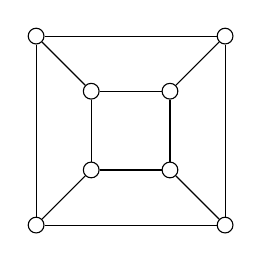
\begin{tikzpicture}[v/.style={circle,draw,fill=white,inner sep=0pt,minimum size=2mm}]
\foreach \x/\y [count=\i] in {0/0,2.4/0,2.4/2.4,0/2.4} \node[v] (o\i) at (\x,\y) {};
\foreach \x/\y [count=\i] in {0.7/0.7,1.7/0.7,1.7/1.7,0.7/1.7} \node[v] (i\i) at (\x,\y) {};
\draw (o1)--(o2)--(o3)--(o4)--(o1);
\draw (i1)--(i2)--(i3)--(i4)--(i1);
\foreach \i in {1,2,3,4} \draw (o\i)--(i\i);
\end{tikzpicture}
\end{center}

\textbf{(B) 對}。 $C_4$ 的頂點依序是 $1, 2, 3, 4$，邊是 $12, 23, 34, 41$。 補圖的邊是原圖沒有的兩條對角線 $13$、$24$，
補圖是兩條不相連的邊。 它的團最大就是一條邊的兩個端點，大小 2（沒有三角形）。

\textbf{(C) 錯}。 強連通元件可以不只一個。 反例：兩個頂點 $u \to v$，$v$ 到不了 $u$，所以 $\{u\}$、$\{v\}$ 是兩個強連通元件
（資結書第~23.1~節）。 只有在整個圖強連通時才剛好一個。

\textbf{(D) 錯}。 反例：3 個頂點、沒有邊的圖，有 3 個連通元件，每個只有 1 個頂點，不到 $3/2$。

\textbf{(E) 對}。 設頂點被分成 $n$ 個團 $Q_1, \ldots, Q_n$（每個頂點恰好在一個團裡）。 取任何一個獨立集 $S$（兩兩不相鄰）：
同一個團裡的兩個頂點一定相鄰，所以 $S$ 在每個 $Q_i$ 裡最多一個頂點，$|S| \le n$。 也就是說，圖裡\textbf{所有}的獨立集
都至多 $n$ 個頂點（最大獨立集大小 $\le$ 團覆蓋數）。 題目說「找得到一個至多 $n$ 個頂點的獨立集」，在這個意義下一定成立
（照字面讀更是顯然：任何一個頂點自己就是）。 \hfill$\blacksquare$
\end{pastsoln}
